% Software Development for Mobile Devices
\documentclass[11pt,english,numbers=endperiod,parskip=half]{scrartcl}

\usepackage{color}
\usepackage{graphicx}
\usepackage{minted}
\usepackage{fancyhdr}
\usepackage{pdflscape}

\pagestyle{fancy}

\rhead{Daniel Parker - 971328X}
\lhead{COS30017 - Software Development for Mobile Devices}

\title{Assignment 04}
\subtitle{COS30017 - Software Development for Mobile Devices}
\author{Daniel Parker 971328X}

\date{\today}

\begin{document}
\maketitle
\thispagestyle{empty}

\section{MetaData App}
\raggedright
The Metadata app contains two activities. The main activity contains a listview of all the ImageData objects and the list item layout is specified in a separate xml layout file. The wiring of these two activities uses the parcelable protocol. The ImageData class implements the Parcelable interface as it is the data that will be sent between the two activities. The EditMetadata activity is called using StartActivityForResult because the edited ImageData object needs to be returned and the updated metadata shown in the listview. The label text sizes are set using styles. The user can change the size of the text by selecting a different option from the dropdown list in the EditMetadata activity, which changes the theme of the activity and subsequently the text size for the labels.
\subsection{What is the Parcelable protocol}
\raggedright
The Parcelable protocol is a method for serializing object data so that it can be sent between activities as context. In the case of this Metadata app, when a user selects an image to edit, the underlying ImageData object is serialized as per the Parcelable interface implementation and sent to the EditMetadata activity. That activity will deserialize the object from using the parcelable interface so that it can be accessed like a normal object and edited. The same is done when the object is returned as a result from the EditMetadata activity. The reason we do not use the Serializable interface is that the Parcelable interface is significantly quicker to serialize and deserialize. This is desirable for Android apps considering that they run on lower powered devices and time is critical with these simple user interface wiring tasks.

\begin{landscape}
\subsection{Source}
\subsubsection{Gallery.java (Startup activity)}
\inputminted{java}{../../Apps/Metadata/app/src/main/java/au/net/danielparker/metadata/Gallery.java}

\subsubsection{EditMetadata.java}
\inputminted{java}{../../Apps/Metadata/app/src/main/java/au/net/danielparker/metadata/EditMetadata.java}

\subsubsection{ImageData.java}
\inputminted{java}{../../Apps/Metadata/app/src/main/java/au/net/danielparker/metadata/ImageData.java}

\subsubsection{activity\_gallery.xml}
\inputminted{xml}{../../Apps/Metadata/app/src/main/res/layout/activity_gallery.xml}

\subsubsection{gallery\_item.xml}
\inputminted{xml}{../../Apps/Metadata/app/src/main/res/layout/gallery_item.xml}

\subsubsection{activity\_edit\_metadata.xml}
\inputminted{xml}{../../Apps/Metadata/app/src/main/res/layout/activity_edit_metadata.xml}

\subsubsection{styles.xml}
\inputminted{xml}{../../Apps/Metadata/app/src/main/res/values/styles.xml}
\end{landscape}

\setlength\fboxsep{0pt}
\setlength\fboxrule{0.5pt}

\section{Usability Test}
\subsection{Objective}
The purpose of this usability test was to identify what label font size felt most comfortable visually for users. It isn't always obvious what users will prefer, but doing a usability test like this one can help to identify the best font size for the situation.
\subsection{Method}
\begin{enumerate}
	\item{The three font sizes were selected by first selecting a font size that looked best in my own opinion. That value was then used as the middle font size and font sizes slightly smaller and larger were selected as the other two font sizes for the usability test.}
	\item{The three selected font sizes were:
		\begin{itemize}
			\item{Small: 10sp}
			\item{Medium: 16sp}
			\item{Large: 22sp}
		\end{itemize}
	}
	\item{The code used three different themes to change the font size. The three themes simple overrode the android value for labelTextSize, which was referenced as the text size for labels using the attribute \textit{android:textSize="?android:attr/labelTextSize"}. The user can then select the size they want within the EditMetadata activity and the theme will be set and activity reloaded.}
\end{enumerate}
\subsection{Participants}
\begin{enumerate}
	\item{
			\begin{itemize}
				\item{Age: 55}
				\item{Occupation: Personal Assistant}
				\item{Computer usage: Daily}
				\item{Smartphone: Owns a smartphone}
			\end{itemize}
		}
	\item{
			\begin{itemize}
				\item{Age: 56}
				\item{Occupation: Software Engineer}
				\item{Computer usage: Daily}
				\item{Smartphone: Does not own a smartphone}
			\end{itemize}
		}
	\item{
			\begin{itemize}
				\item{Age: 24}
				\item{Occupation: Waitress}
				\item{Computer usage: Once a month}
				\item{Smartphone: Owns a smartphone}
			\end{itemize}
		}
\end{enumerate}
\subsection{Results}
\subsubsection{Participant 1}
\begin{table}[H]
	\begin{tabular}{| p{0.55\linewidth} | p{0.15\linewidth} | p{0.15\linewidth} | p{0.15 \linewidth} |}
		\hline
			&	Small	&	Medium	&	Large \\ \hline
		Can you read the text?	& Only Just	& Yes	& Yes \\ \hline
		Do you prefer this font size for the labels? & No & Yes & No \\ \hline
		Do you prefer this font size for the information display? & No & Yes & No \\
		\hline
	\end{tabular}
\end{table}

\subsubsection{Participant 2}
\begin{table}[H]
	\begin{tabular}{| p{0.55\linewidth} | p{0.15\linewidth} | p{0.15\linewidth} | p{0.15 \linewidth} |}
		\hline
			&	Small	&	Medium	&	Large \\ \hline
		Can you read the text?	& No & Yes	& Yes \\ \hline
		Do you prefer this font size for the labels? & No & Yes & No \\ \hline
		Do you prefer this font size for the information display? & No & Yes & Yes \\
		\hline
	\end{tabular}
\end{table}

\subsubsection{Participant 3}
\begin{table}[H]
	\begin{tabular}{| p{0.55\linewidth} | p{0.15\linewidth} | p{0.15\linewidth} | p{0.15 \linewidth} |}
		\hline
			&	Small	&	Medium	&	Large \\ \hline
		Can you read the text?	& Yes	& Yes	& Yes \\ \hline
		Do you prefer this font size for the labels? & No & Yes & No \\ \hline
		Do you prefer this font size for the information display? & No & Yes & No \\
		\hline
	\end{tabular}
\end{table}

\subsection{Recommendation}
The recommendation from the results of the usability test is that the Medium 16sp font size is used for labels and information display. This is due to all of the tested users saying that they could read and preferred that size for the label and display information text.

\subsection{Reflection}
If the usability test were to be run again, the users would be show all the fonts first and then asked to only give one preferred out of the three fonts for the labels and display information.

%\centering{
%	\fbox{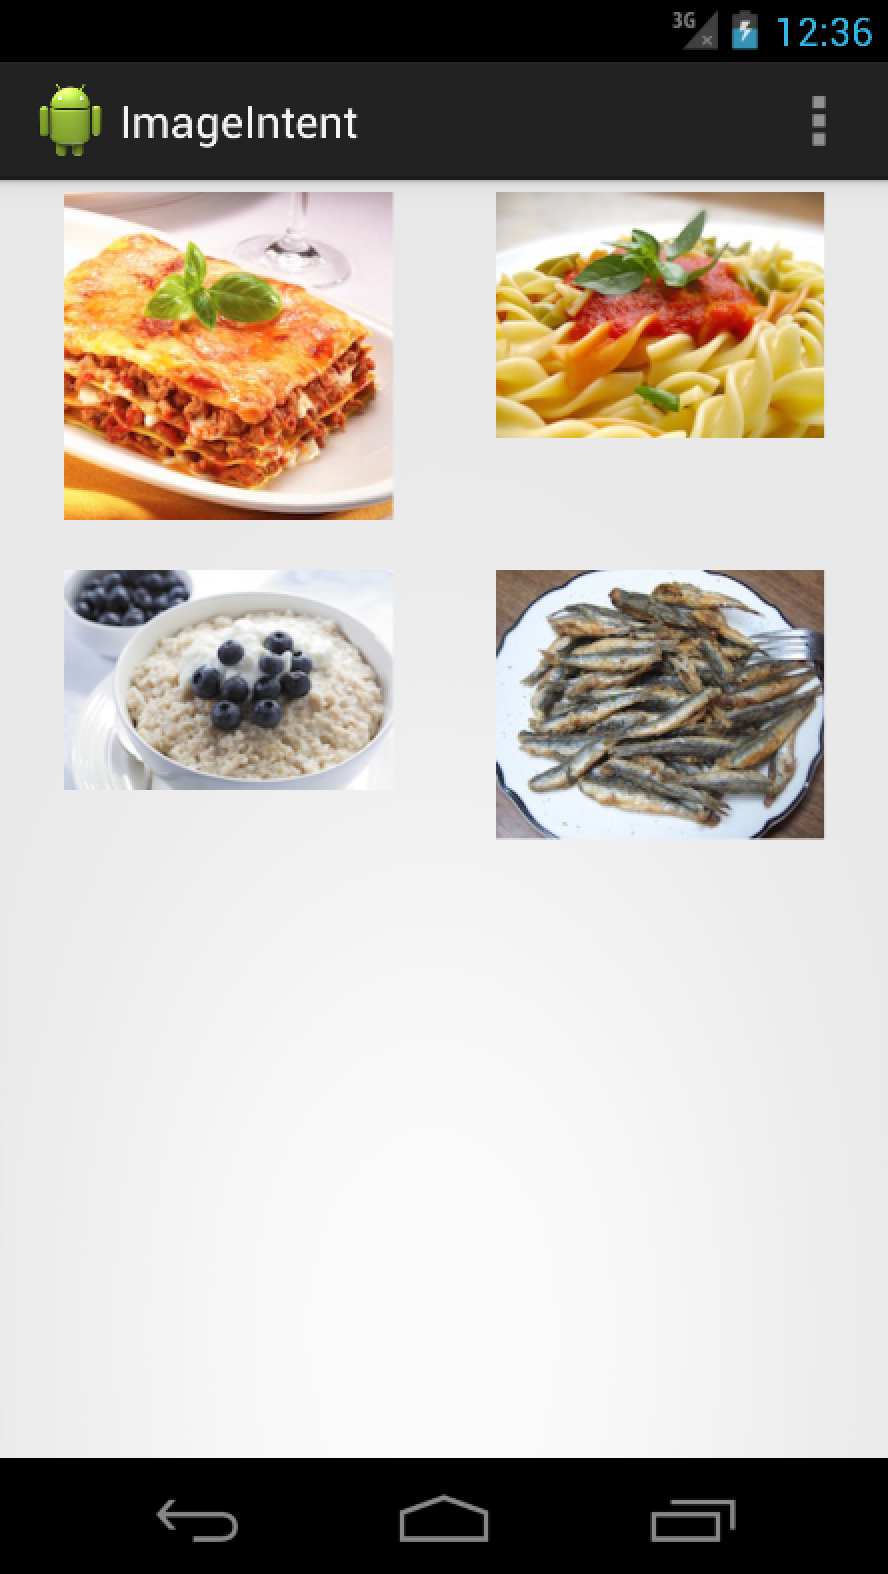
\includegraphics[width=5cm]{images/gallery.png}}
%}\\
%\bigskip
\end{document}
